%%%%%%%%%%%%%%%%%%%%%%%%%%%%%%%%%%%%%%%%%%%%%%%%%%%%%%%%%%%%%%%%%%%%%
%%%%%%%%%%%                   PROBLEM 1                   %%%%%%%%%%%
%%%%%%%%%%%%%%%%%%%%%%%%%%%%%%%%%%%%%%%%%%%%%%%%%%%%%%%%%%%%%%%%%%%%%

\section{پرسش اول}
به سوالات پرسیده شده در مورد متودولوژی FDD
\LTRfootnote{Feature Driven Development}
پاسخ می‌دهیم:
\begin{enumerate}[i]
\item 
متودولوژی FDD یک متودولوژی مدل رانه
\LTRfootnote{Model Driven}
با Iteration های کوتاه است که هدف آن ارائه‌ی نرم افزار مشخص و کارا در بازه‌های زمانی متناسب و مشخص است.

این متودولوژی یک فرایند ویژگی 
\LTRfootnote{Feature}
محور است. یک Feature قطعه‌ی کوچکی از کارایی مورد نظر و دارای ارزش از نظر کارفرما است که به صورت 
\lr{<Action> <Result> <Object>}
توصیف می‌شود (مانند \lr{Backup the files of current user}).

زمان مورد نیاز برای اتمام هر ویژگی نباید بیشتر از ۲ هفته به طول بیانجامد. در این صورت ویژگی مورد نظر باید به چند ویژگی حداکثر ۲ هفته‌ای شکسته شود.

در این متودولوژی برای توسعه‌ی هر ویژگی و پیگیری پیشرفت پروژه یک milestone تعیین می‌شود. توسعه‌ی توسط این مدل از ۵ فعالیت تشکیل شده است. 

طی دو فعالیت اول که به صورت متوالی انجام می‌شوند، صورت مدل کلی پروژه تهیه و تثبیت می‌شود و ۳ فعالیت نهایی به صورت تکراری برای پیاده سازی هر ویژگی انجام می‌شوند.

مراحل مدلسازی عبارتند از:
\begin{enumerate}
\item 
\textbf{توسعه‌ی مدل کلی پروژه:} \newline
در ابتدای پروژه به دامنه و محیط پروژه به صورت سطح بالا پرداخته می‌شود و مورد بررسی قرار می‌گیرند. در این مرحله برای واضح شدن نیازمندی‌های سیستم در صورت لزوم به مطالعه‌ی مستندات و منابع پرداخته می‌شود.

در ادامه مدل‌های دقیق تر برای هر ناحیه‌ی مدلسازی توسط گروه‌های مدلسازی تهیه شده و به صورت تیمی مورد بازبینی و بررسی قرار می‌گیرند. در صورت لزوم پروسه‌ی ویرایش و بازبینی تا نهایی شدن مدل‌ها تکرار می‌شود. به همراه مدلسازی یادداشت‌هایی در جهت ثبت جزئیات مدل‌ها نوشته شده و در کنار مدل ثبت می‌شوند.


در نهایت مدل‌های کوچکتر ناحیه بندی شده با هم ادغام شده و یک مدل نهایی را ایجاد می‌کنند.

\item
\textbf{ایجاد لیست ویژگی‌ها:} \newline
در ادامه اطلاعات و دانش به دست آمده در مرحله‌ی اول مدلسازی برای تولید یک لیست از ویژگی‌های مورد تصور برای سیستم مورد استفاده قرار می‌گیرد.

برای این منظور دامنه‌ی مساله‌ی مورد بررسی در پروژه را به بخش‌های مختلف تقسیم کرده، فعالیت‌های کسب و کار در هر یک از این بخش‌ها و مراحل آنها را برای تشکیل لیست ویژگی‌های سیستم مورد بررسی قرار می‌دهیم.
\end{enumerate}
 
در نهایت پس از این مراحل مدل‌سازی، برای هر یک از ویژگی‌ها، مراحل برنامه‌ریزی، طراحی و پیاده سازی انجام می‌پذیرد.
 \cite{wikipedia-fdd}
 
\item
خیر این میزان از مدلسازی ناقض چابکی نیست. ابتدا فلسفه‌ی توسعه‌ی چابک منافاتی با مدلسازی ندارد و صرفا از مدلسازی بیش از حد و دست و پا گیر بازداری می‌کند.  از طرفی دیگر "هدف اصلی متودولوژی FDD ارائه‌ی نرم افزار ملموس و کارا در بازه‌های زمانی مشخص"
\cite{wikipedia-fdd}
 است که این همان هدف اصلی توسعه‌ی چابک است.

اجایل بودن به معنی دست و پا بند نبودن مستندات و قرارداد‌ها و سایر سند‌هاست و هرگز به معنی حذف کامل آنها نیست.


جالب است بدانیم که متودولوژی FDD قبل از بیانیه‌ی توسعه‌ی چابک ایجاد شده و در آن موقع نیز به نکات اصلی آن توجه داشته است!
\cite{why-fdd-is-agile}

\end{enumerate}

\begin{center}
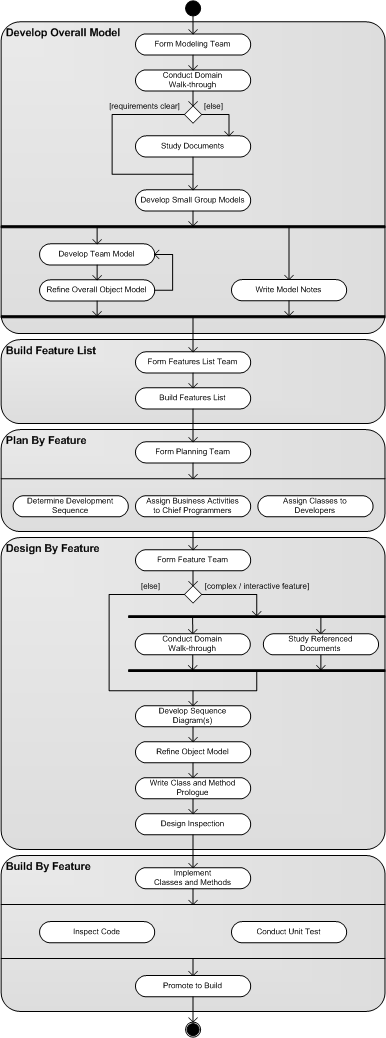
\includegraphics[width=0.5\textwidth]{images/Fdd_process_diagram}

منبع تصویر: ویکی‌پدیا
\LTRfootnote{\url{https://en.wikipedia.org/wiki/File:Fdd_process_diagram.png}}
\end{center}

